%%%%%%%%%%%%%%%%%%%%%%%%%%%%%%%%%%%%%%%%%%%%%%%%%%%%%%%%%%%%%%%%%%%%%%%%%%%%%%%%
%2345678901234567890123456789012345678901234567890123456789012345678901234567890
%        1         2         3         4         5         6         7         8

\documentclass[letterpaper, 10 pt, conference]{ieeeconf}  % Comment this line out if you need a4paper

% \documentclass[letterpaper, 12 pt, twoside]{report}  % Comment this line out if you need a4paper


%\documentclass[a4paper, 10pt, conference]{ieeeconf} % Use this line for a4 paper able to be

\IEEEoverridecommandlockouts %This command is only needed if you want to use the \thanks command

\overrideIEEEmargins  % Needed to meet printer requirements.

%In case you encounter the following error:
%Error 1010 The PDF file may be corrupt (unable to open PDF file) OR
%Error 1000 An error occurred while parsing a contents stream. Unable to analyze the PDF file.
%This is a known problem with pdfLaTeX conversion filter. The file cannot be opened with acrobat reader
%Please use one of the alternatives below to circumvent this error by uncommenting one or the other
%\pdfobjcompresslevel=0
%\pdfminorversion=4

% See the \addtolength command later in the file to balance the column lengths
% on the last page of the document

% The following packages can be found on http:\\www.ctan.org
\usepackage{graphicx} % for pdf, bitmapped graphics files
%\usepackage{epsfig} % for postscript graphics files
%\usepackage{mathptmx} % assumes new font selection scheme installed
%\usepackage{times} % assumes new font selection scheme installed
\usepackage{amsmath} % assumes amsmath package installed
\usepackage{amssymb}  % assumes amsmath package installed
%\usepackage{dsfont}
\usepackage{algorithm}
\usepackage{algorithmic}
\usepackage{commath}
\usepackage[bottom]{footmisc} %allows for footers to be used with \footnote

\usepackage{url} %These are to break up the urls in the bibliography so they dont hang over the margin
\def\UrlBreaks{\do\/\do-}
% \usepackage{breakurl} %doesnt seem to be needed, but I left it here just in case
\usepackage[breaklinks]{hyperref}

\usepackage{xcolor} %custom commands for annotation while drafting
\newcommand{\todo}[1]{{\color{blue}[TODO: #1]}}
\newcommand{\comment}[1]{{\color{red}[COMMENT: #1]}}
\newcommand{\response}[1]{{\color{green}[RESPONSE: #1]}}

\graphicspath{{figures/}}

\DeclareMathOperator*{\argmax}{arg\,max}
\DeclareMathOperator*{\argmin}{arg\,min}


\title{\LARGE \bf
Multi-Agent Mapping and Navigation of Unknown GPS-Denied Environments Using a Relative Navigation Framework}

\author{Jacob M. Olson$^{1}$, Nathan A. Toombs, Timothy W. McLain$^{2}$% <-this % stops a space
\thanks{$^{1}$The corresponding author can be contacted at
        {\tt\small jacobmo at byu.edu}.}%
\thanks{$^{2}$All authors are with the Department of Mechanical Engineering,
        Brigham Young University, Provo, UT, 84602, USA.}%
% \thanks{Thanks to Mathieu Labbe for being responsive to answering questions on the RTAB-Map forum and helping with developing the map merging node.}%
}

\begin{document}

\maketitle
\thispagestyle{empty}
\pagestyle{empty}

\graphicspath{{figures/}}

%%%%%%%%%%%%%%%%%%%%%%%%%%%%%%%%%%%%%%%%%%%%%%%%%%%%%%%%%%%%%%%%%%%%%%%%%%%%%%%%
\begin{abstract}

When generating 3D maps with unmanned aerial vehicles (UAVs) in GPS-denied environments, it is important to correctly handle path planning, estimation, and mapping techniques. Because multirotor UAVs are limited in flight time, using multiple UAVs to map an environment collaboratively can significantly improve the mapping efficiency. This paper addresses the following key issues required to enable mapping with multiple agents: Combining a reactive path planner with an obstacle avoidance algorithm to handle navigation in complex environments. Estimating the relative and global states of a UAV separately with a relative navigation framework to allow for loop closures in the mapping process without causing the estimation to diverge. Adapting a graph-based simultaneous localization and mapping (graph-SLAM) technique for multiple UAVs flying simultaneously and merging their maps in real-time. We were able to use these strategies to generate dense maps in complex GPS-denied environments with multiple UAVs.

\end{abstract}

\section{Introduction}

\footnote{The following chapter is composed from paper "Multi-Agent Mapping and Navigation of Unknown GPS-Denied Environments Using a Relative Navigation Framework" to be submitted to ICUAS 2020} Many new applications are being explored to make use of dense 3D mapping technology, such as surveying an earthquake damaged building to find survivors and check for damage, infrastructure inspections, and generating as-built models for infrastructure. Mapping and navigating an environment such as these, where global positioning system (GPS) signals are degraded or entirely unavailable, are difficult. Often, these GPS-denied environments are inaccessible to ground robots due to rubble or structural damage. Environments like these lend themselves better to the use of unmanned aerial vehicles (UAVs) to carry out some or all of the mapping. When navigating indoor environments with a UAV, collision with any obstacles can be catastrophic and measures must be taken to avoid them. We use a combination of a high-level reactive path planner and a low-level obstacle avoidance filter to avoid collisions.


Most dense mapping approaches rely on high-quality GPS measurements to geotag data to enable map generation \cite{Siebert2014, Martin2015}. These methods break down when GPS is not available because the global position must be estimated rather than measured. To overcome the lack of GPS, some form of simultaneous localization and mapping (SLAM) with visual odometry can be used. We use a form of graph-SLAM with a 3D camera and depth-enhanced visual odometry.

Because of the limited flight time of UAVs, mapping large areas with a single UAV can be inefficient. The mapping process can be streamlined by dividing the area between multiple UAVs and then, combining their individual maps into a single combined map. One recent approach to this problem by Michael et al. used ground robot and a UAV to collaboratively map an earthquake-damaged building. In this research, the UAV acted as an extension to the ground robot, flying into the difficult terrain to build onto the map started by the ground robot \cite{Michael2012}. More recently, Mangelson et al. detailed a method to effectively merge maps collected from multiple robots acting separately after the mapping process is complete \cite{Mangelson2018}. In our approach, we use multiple UAVs flying simultaneously to map an indoor GPS-denied environment. The method we propose also combines the maps from the UAVs into a single map in near real-time.

The remainder of the paper is organized as follows: Section \ref{nav_approach} presents the framework we use to navigate and map an environment along with background information about previous work that we build upon. Section \ref{nav_planning} details the planning and control schemes used to successfully navigate an unknown environment. The method used to combine maps in near real-time is then explained in Section \ref{nav_merge}. Results showing and evaluating the generated maps are presented in Section \ref{nav_results}. Finally, conclusions are presented in Section \ref{nav_conclusions}.

%%%%%%%%%%%%%%%%%%%%%%%%%%%%%%%%%%%%%%%%%%%%%%%%%%%%%%%%%%%%%%%%%%%%%%%%%%%%%%%%
\section{Technical Approach}\label{nav_approach}

\subsection{Problem Statement}

For UAV-based map building to be successful, flight paths that produce high-quality loop closures and sufficient coverage of the environment are required. The framework presented in this section assumes that these high-quality paths will be supplied either by the user or by a high-level coverage path planner. Rather than focus on high-level path generation, the focus of this paper is first, to show that properly estimating UAV states allows for successful GPS-denied navigation, and second, to demonstrate how to streamline the mapping process by merging multiple maps into a single one. A high-level network diagram is shown in Fig. \ref{fig:rtab_network} that outlines the framework we use to successfully generate a single merged map from multiple UAVs in a GPS denied environment.

\begin{figure*}
\centering
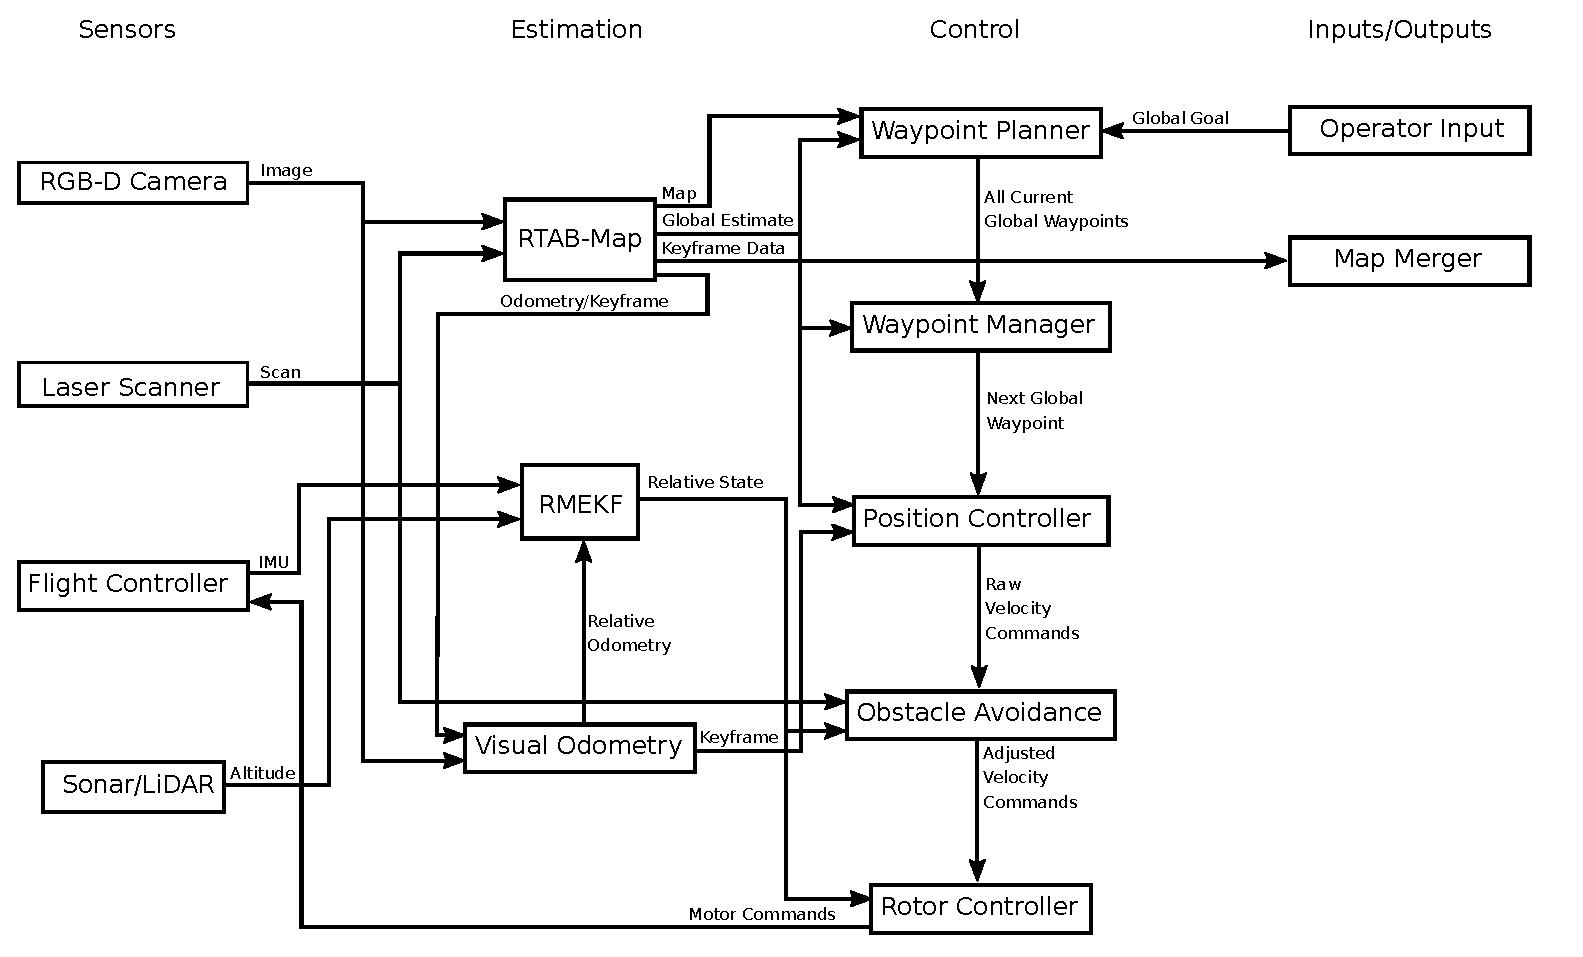
\includegraphics[width=1.0\linewidth]{rtab_relative_nav_network}
\caption{The network diagram of the relative navigation framework proposed in this paper.}
\label{fig:rtab_network}
\end{figure*}

\subsection{Sensors}

Since we are operating in a GPS-denied environment, we are not able to rely on GPS measurements to give us global information about the UAVs locations. The sensors used by each UAV to estimate their states are a 3D color and depth (RGB-D) camera (Intel RealSense D435 \cite{Intel}), a planar light detection and ranging (LiDAR) laser scanner, a single-beam LiDAR range finder, and an inertial measurement unit (IMU) on the onboard flight controller. Using only these sensors and the flight computer, we estimate the states of the UAV with sufficient accuracy to control its attitude and position. The following section elaborates on how these sensors are used in the estimation.

\subsection{Estimation}

Estimation is the most critical element in enabling autonomous flight. Without adequate position and attitude estimation, autonomous navigation algorithms have difficulty. We use a graph-SLAM approach similar to that developed by Thrun et al. \cite{Thrun2006} to navigate and generate the maps. Loop closures, which occur when a robot sees the same objects from similar locations at different points in time, can cause estimators to diverge if they are not handled correctly. Every time a new loop closure occurs, the map and position estimate are re-optimized. If the new loop closure results in a large shift in the current position estimate, a naive estimator can diverge because of the discontinuity of the estimated global position. To avoid the issue of loop closures causing instability in the controller, we estimate the global and relative states of the UAV separately and do not rely on the global state estimate to control the attitude of the UAV.

We store the current global state estimates in a transformation tree as shown in Fig. \ref{fig:tf_tree}. The $\mathit{world}$ frame is the inertial NED (north-east-down) frame with a fixed origin that does not change over time. The UAV's starting location with respect to the world is set as the $\mathit{map}$ frame which is represented in the inertial NWU (north-west-up) orientation. The $\mathit{base\_link}$ frame represents the current estimated position of the the UAV in the NED orientation with the $\mathit{camera\_link}$ frame representing the position in the NWU orientation. The $\mathit{camera\_base\_link}$ frame represents the current position of the camera in the camera frame.

\begin{figure*}
\centering
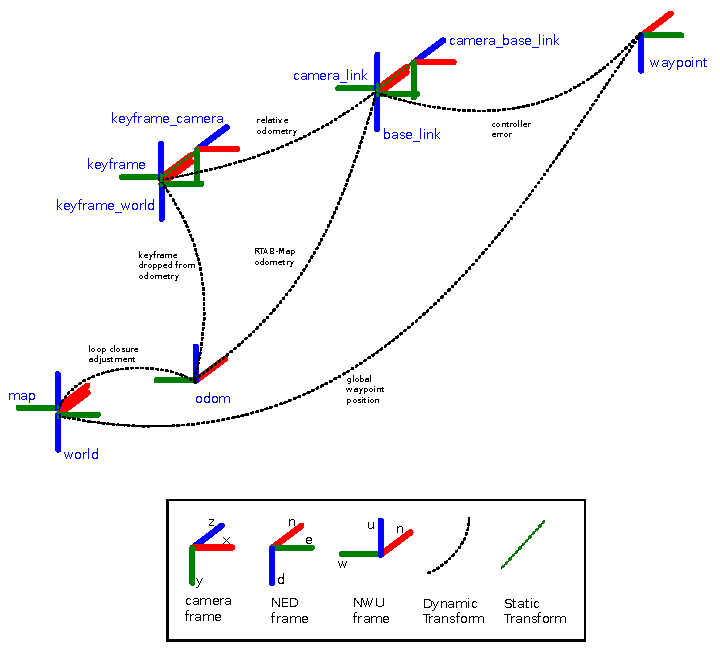
\includegraphics[width=0.9\linewidth]{tf_tree_relative_rtab}
\caption{The transformation tree of the reference frames used in estimation and control.}
\label{fig:tf_tree}
\end{figure*}

The $\mathit{odom}$ frame is used to adjust for loop closures. When the flight begins, the $\mathit{odom}$ frame starts with zero offset from the $\mathit{map}$ frame. Every time a loop closure is detected and the map is re-optimized, the transform between the $\mathit{map}$ and $\mathit{odom}$ frames is adjusted to reflect the correction in the current global state estimate. This allows the transform between the $\mathit{odom}$ frame and the robot frames ($\mathit{camera\_link}$ and $\mathit{base\_link}$) to stay continuous when loop closures are detected even though the position estimate does not.

The $\mathit{keyframe}$, $\mathit{keyframe\_world}$ and $\mathit{keyframe\_camera}$ frames are used to track the relative visual odometry used by the relative estimator. More specifically, the relative visual odometry is stored in the tree as the transform between the $\mathit{keyframe}$ and $\mathit{camera\_link}$ frames in the NWU orientation. For convenience, we also keep track of the the NED orientation with the $\mathit{keyframe\_world}$ frame and the camera orientation with the $\mathit{keyframe\_camera}$ frame.

The UAV's current waypoint is represented as the transform between the $\mathit{world}$ and $\mathit{waypoint}$ frames. This way, a loop closure does not shift the desired global position of the waypoint. The position controller operates on the error between the $\mathit{waypoint}$ and $\mathit{base\_link}$ frames. More detail regarding the uses and implementations of these transforms will be further explained in the following sections.

%This is under the assumption that the desired waypoint location is known globaly, this could be modified to set the new waypoint relative to odom frame if the position is relative to the current obstacles rather than the global position.

\subsubsection{RTAB-Map}

The real-time appearance-based mapping (RTAB-Map) package, developed by Labbe et al. \cite{Labbe2011a,Labbe2013,Labbe2019}, is a powerful open-source software library. It uses graph-SLAM with appearance-based loop closures to generate high-quality, dense 3D maps using only a RGB-D camera and a planar laser scanner. When coupled with the depth-enhanced visual odometry algorithm called RGBD-Odometry, which was developed in conjunction with RTAB-Map \cite{Labbe2019}, the UAV's position with respect to the map that is being built can be accurately estimated at all times. The map-building algorithm uses a keyframe-based approach. Unlike the visual odometry algorithm, the map-building algorithm does not try to use the information from every camera frame to build the map and optimize the graph. Instead, it only uses camera information that has been saved periodically at a set rate. In our case, once every second the information from the current camera frame is sent to RTAB-Map and saved as a keyframe. Only these keyframes are used to build the map and optimize the graph. RTAB-Map is primarily designed for use with slow-moving ground robots that do not need high-rate state estimation to work. The only state estimation that is performed by RTAB-Map is from the visual odometry, which is limited by the frame rate of the camera. We found the estimation rate of RTAB-Map on our hardware to be in the 10-30 Hz range, which is not sufficient for autonomous navigation of a UAV. We use the state estimates from the RGBD-Odometry node as an input to the estimation for the relative framework.

Although the current functionality of RTAB-Map does allow for a single robot to combine maps from multiple sessions, it does not allow for multiple agents mapping simultaneously to combine the maps into a single one. This paper proposes a method to extend the functionality of RTAB-Map to combine the maps of multiple agents flying simultaneously into a single map in near real-time. The implementation of this method is detailed in Section~\ref{nav_merge}.

RTAB-Map manages the $\mathit{map}$, $\mathit{odom}$, $\mathit{base\_link}$, $\mathit{camera\_link}$, and $\mathit{camera\_base\_link}$ frames in the transformation tree as previously described. Along with the frames, it handles all of the loop closures and graph optimization. We use the current position estimate produced by RTAB-Map for the position controller and waypoint manager. Because of the inevitable inaccuracies and the lower estimation rates of RTAB-Map, we do not use these estimates to perform attitude control on the UAVs. Rather, we use a relative navigation framework to estimate the relative state and control the attitude.

\subsubsection{Visual Odometry} \label{vis_odom}

The odometry and keyframe information generated by RTAB-Map is used to produce a relative odometry message that is sent to the relative estimator. RTAB-Map produces a global visual odometry that provides a real-time estimate of the global position and orientation of the UAV. Each time a new keyframe is declared, a new node is added to the graph, and the visual odometry node shown in Fig \ref{fig:rtab_network} resets the transform between the $\mathit{keyframe}$ and $\mathit{camera\_link}$ frames to zero. The relative odometry only tracks the UAV's movement with respect to the last keyframe that was declared and stores the information as the transform between the $\mathit{keyframe}$ and $\mathit{camera\_link}$ frames. Because of the continual resetting of the keyframe transform, the odometry used by the relative estimator is less susceptible to drift over time \cite{Leishman2014relative}.

\subsubsection{RMEKF}

The relative navigation framework \cite{Wheeler2017,Wheeler2018,Koch2017} has been shown to successfully estimate the UAV's relative state sufficient to autonomously navigate in GPS-denied environments that have previously been mapped. Thus far, however, it has not been extended to estimation and navigation in unknown and unmapped environments. This paper proposes a method to extend the functionality to these environments.

The relative multiplicative extended Kalman filter (RMEKF) is the heart of the relative framework. It uses the IMU measurements from the flight controller, the relative visual odometry explained previously, and the attitude measurement from the LiDAR single-beam range finder for the measurement updates. Then, using a multirotor dynamics model, the RMEKF accurately estimates the relative state of the UAV with respect to the previous keyframe. This estimate is used for obstacle avoidance and high-rate attitude control. The RMEKF makes no effort to estimate the global position of the UAV. As a result, corrections in the estimated global position from loop closures and drift in visual odometry do not cause the estimator to diverge. This enables the UAV to avoid stability issues in the velocity and attitude controllers.

\subsection{Control}

To successfully control a UAV using the relative navigation framework, the control must be segmented into different tiers to take advantage of both global and relative estimates. The following paragraphs explain the different tiers of the the UAV control shown in Fig \ref{fig:rtab_network}.

\subsubsection{Waypoint Planner}

The first stage of the control architecture is the waypoint planner. The inputs to the planner are the global goal, the current known obstacles, and the current global estimates. It outputs a path to the goal that avoids all known obstacles as set of waypoints. The detailed workings of the planner will be further explained in Section~\ref{nav_planning}.

\subsubsection{Waypoint Manager}

After receiving the waypoints, the waypoint manager selects the appropriate waypoint for the UAV and sends the global location to the position controller. The waypoint manager monitors the position and heading error between the current estimated position and the current waypoint. When the error decreases below a user-defined threshold value, the next waypoint is sent to the position controller.

\subsubsection{Position Controller}

The position controller drives the error between the current estimated position and heading of the UAV and the next waypoint to zero. Since it operates in the error space of the the UAV rather than the state space, sudden shifts in the UAV's position estimate caused by loop closures have minimal effect on the controller. When these shifts happen, the controller is able to quickly adjust continue controlling the error to zero. The position controller outputs a velocity command.

\subsubsection{Obstacle Avoidance} \label{obs_avoid}

Before passing the velocity command into the attitude controller, it is filtered through an obstacle avoidance algorithm. This algorithm uses the current relative estimates from the RMEKF and current obstacles detected by the planar laser scanner to modify the input velocity command. It uses a cushioned extended-periphery avoidance (CEPA) technique \cite{Jackson2016} to alter the velocity command when necessary by pushing the UAV away from obstacles while changing the incoming velocity command as little as possible. Because the position controller does not manage the trajectory of the UAV, it often causes overshoot after reaching waypoints. This overshoot is suppressed by the CEPA filter if it causes the UAV to fly near obstacles. The obstacle avoidance node then sends the modified velocity command to the attitude controller.

\subsubsection{Attitude Controller}

The attitude controller is a conventional PID controller that runs on the autopilot. It takes the linear velocity from the position controller as the input commands, performs the attitude control loop, and outputs the raw motor commands to the electronic speed controllers (ESCs).

\subsection{Inputs/Outputs}

The input for each agent in the system is the desired high-level path either from operator input or from a high-level path planner. As each agent maps the environment, keyframe data consisting of the color and depth images and the  feature descriptions from the images is sent to the map merger each time a new keyframe is declared. The map merger will be further explored in Section~\ref{nav_merge}.

%%%%%%%%%%%%%%%%%%%%%%%%%%%%%%%%%%%%%%%%%%%%%%%%%%%%%%%%%%%%%%%%%%%%%%%%%%%%%%%%
\section{Planning}\label{nav_planning}

When designing the reactive planner, we explored using both node-based optimal algorithms and sampling based algorithms \cite{Yang2016}. Node-based (or heuristic search) algorithms like A* work well to find optimal paths around obstacles \cite{Nilsson2011}. The downside to these planners is that in order to find a path, they need to exhaustively search the design area. This makes them less efficient to use when the map is large and constantly changing. They also require the environment to be discretized, which can result in the planner not finding paths to the goal when a path does exist. This tends to happen in complex maps when the environment is coarsely discretized. Sampling-based algorithms, like rapidly-exploring random trees (RRT) \cite{Lavalle1998} are effective for planning in real-time with dynamic obstacles. RRT randomly searches the full, non-discretized map for feasible paths rather than requiring an exhaustive search. Although RRT does not guarantee optimal paths, it is much less computationally intensive than A* each time a new path is planned. More recently, improvements to RRT have been explored such as RRT* \cite{Karaman2011}, which generates asymptotically optimal paths by modifying the search tree. Since our planner is used as a form of exploration of unknown environments, we chose to use RRT. This allows the flight path to be more random and encourage more exploration of the map while flying paths.

We used a form of RRT with a path smoothing approach similar to that proposed \cite{Beard} to improve and simplify the resultant paths. Since our planner uses a dense 2D grid map of all currently known obstacles, some adjustments are needed to efficiently plan and re-plan when new obstacles are discovered in the current path.

\subsection{Global Goal Following with Relative Estimation}

As mentioned earlier, the relative estimator critical to keeping the UAV airborne only estimates the UAV's relative state with respect to the last keyframe and makes no attempt to estimate the global position of the UAV. By doing so, the global estimate of the position does not have to be continuous and is able to slide and adjust with loop closure corrections without affecting the estimator. The path planner generates a global path from the current position to the goal. The global paths do not adjust with loop closures and the map is continually changing as the UAV flies. For both of these reasons, obstacles can appear in the path at any time. To avoid these obstacles, the planner dynamically re-plans any time an obstacle is detected in the path.

\subsection{Reactive Path Planning}

Fig. \ref{fig:reactive_plan} shows the process of how the dynamic path planner works in an example scenario. When the UAV starts, little is known about the environment. The only obstacles in the map are the ones that are within line-of-sight of the laser scanner when the flight begins. A path is planned to the goal that avoids the obstacles that are initially detected. As the UAV flies, the obstacle map is continuously updated with new obstacles and the path is constantly being checked for collisions. If collisions are found, a new path is planned to the goal from the current location that avoids the newly discovered obstacles. This process continues until the agent successfully reaches the goal. Since the path is updated any time a potential collision is detected, no prior knowledge of the environment is required to begin flying.

\begin{figure*}
\centering
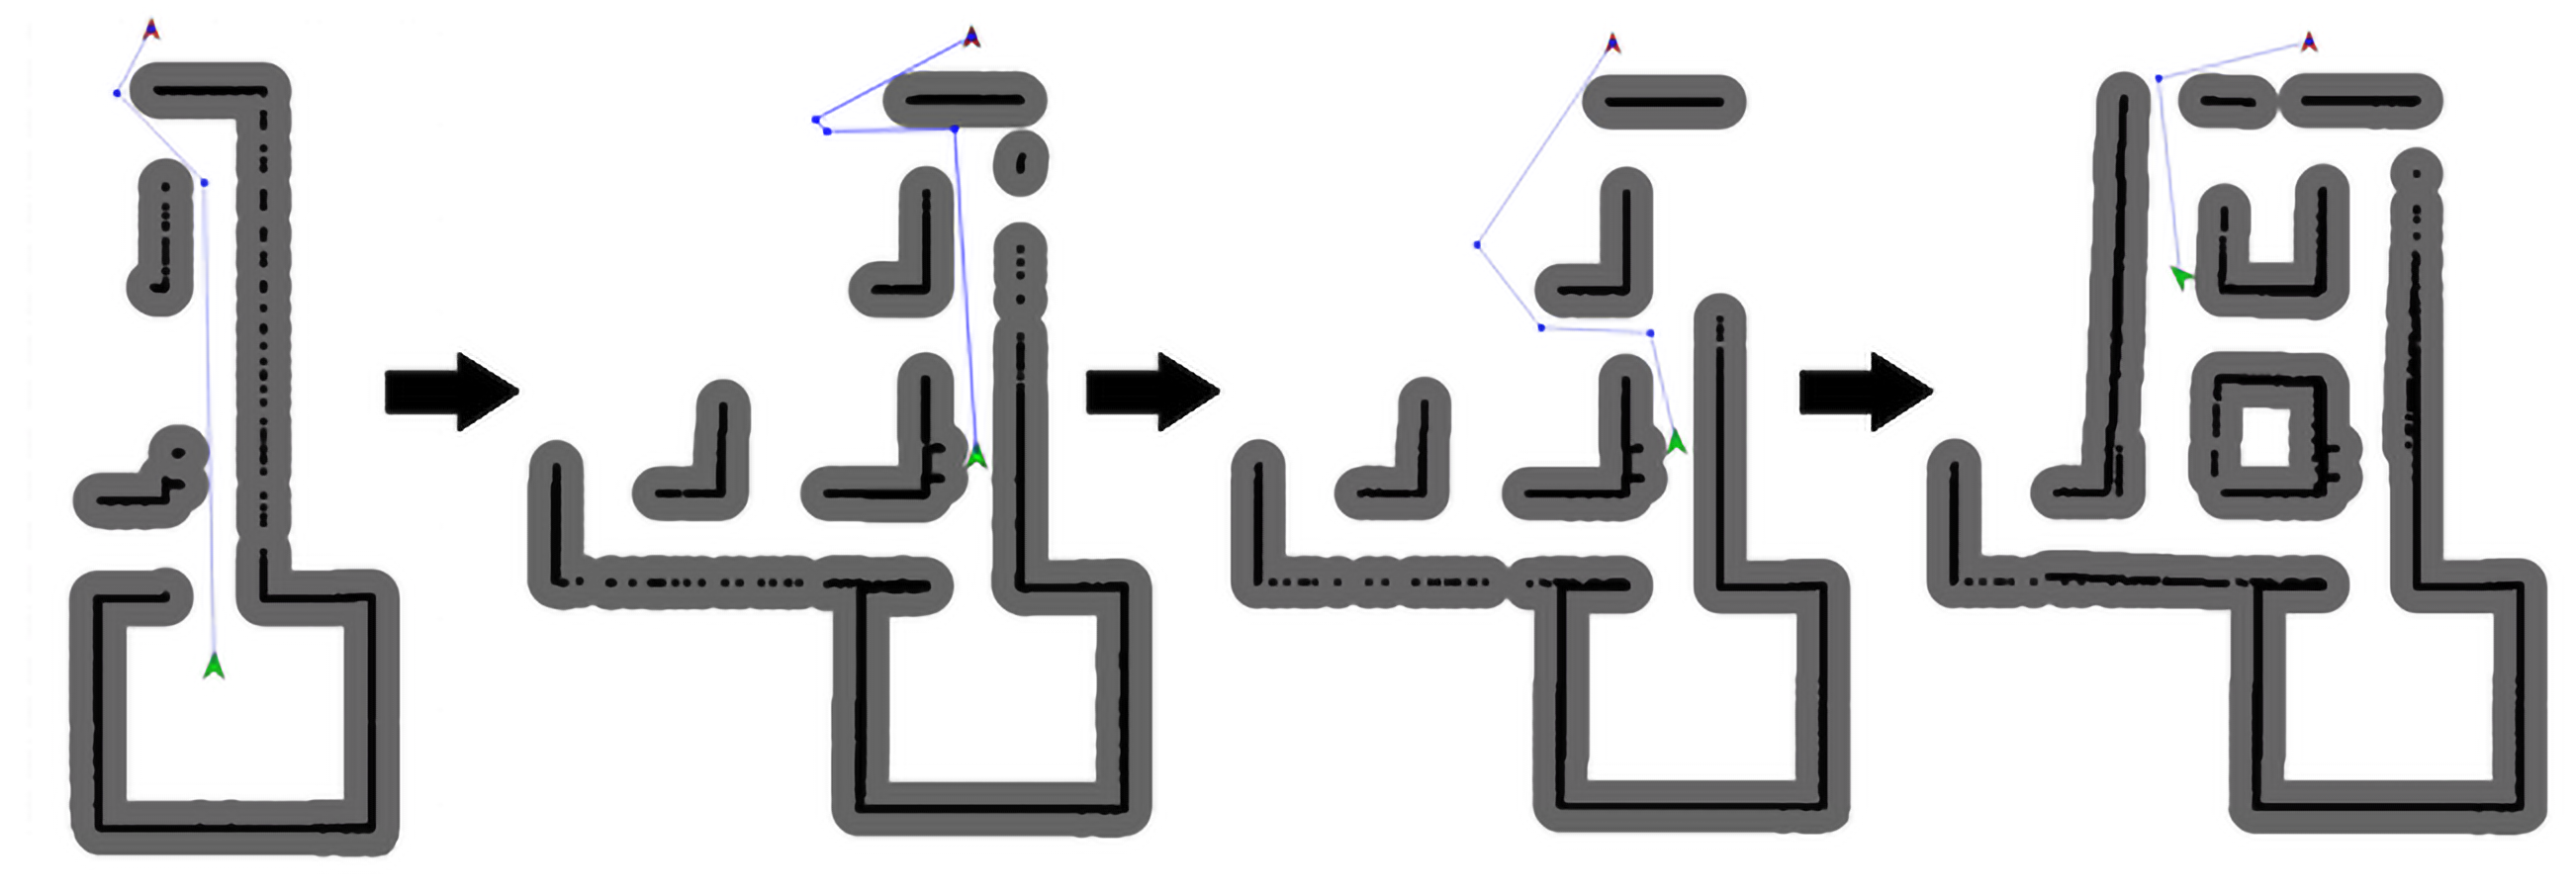
\includegraphics[width=1.0\linewidth]{adaptive_path_plan2.png}
\caption[An example of how the reactive path planner works.]{An example of how the reactive path planner works as the UAV flies the planned path. The current estimated position is marked by the green arrow, the current goal position is marked by the red arrow, and the current path is marked with blue lines. Detected obstacles and safety buffers are represented with black and grey respectively.}
\label{fig:reactive_plan}
\end{figure*}

The planner also includes a buffer around each detected obstacle to avoid planning paths that would cause the UAV to fly too close to the obstacles. The buffer size is set by the user, but is always at least half the width of the UAV. This ensures that every waypoint is sufficiently far from obstacles that it can be reached without any part of the UAV touching an obstacle.

Since this planner is used in conjunction with the CEPA obstacle avoidance node explained in \ref{obs_avoid}, the UAV can effectively navigate through complex maps and avoid obstacles in emergency situations. The planner enables complex navigation that would not be possible with only obstacle avoidance. The obstacle avoidance node filters velocity commands from the position controller that would inadvertently cause the UAV to collide with obstacles when either a new obstacle is detected that is not in the current map, or when the position controller causes overshoot.

\subsubsection{Efficient Collision Detection}
Most implementations of RRT are not designed to deal with extremely large number of obstacles. The obstacles we use are from a 2D grid map generated by RTAB-Map based on the planar LiDAR scanner returns. Consequently, rather than having just a few large obstacles, there are many small obstacles. Using a standard obstacle detection check with each propagation of the RRT would be extremely inefficient. To maximize the efficiency during planning, we use a strategy that allows the planner to ignore most obstacles in the map when performing collision checks. An example of how this works is illustrated in Fig.~\ref{fig:rrt_sample}.

\begin{figure}
\centering
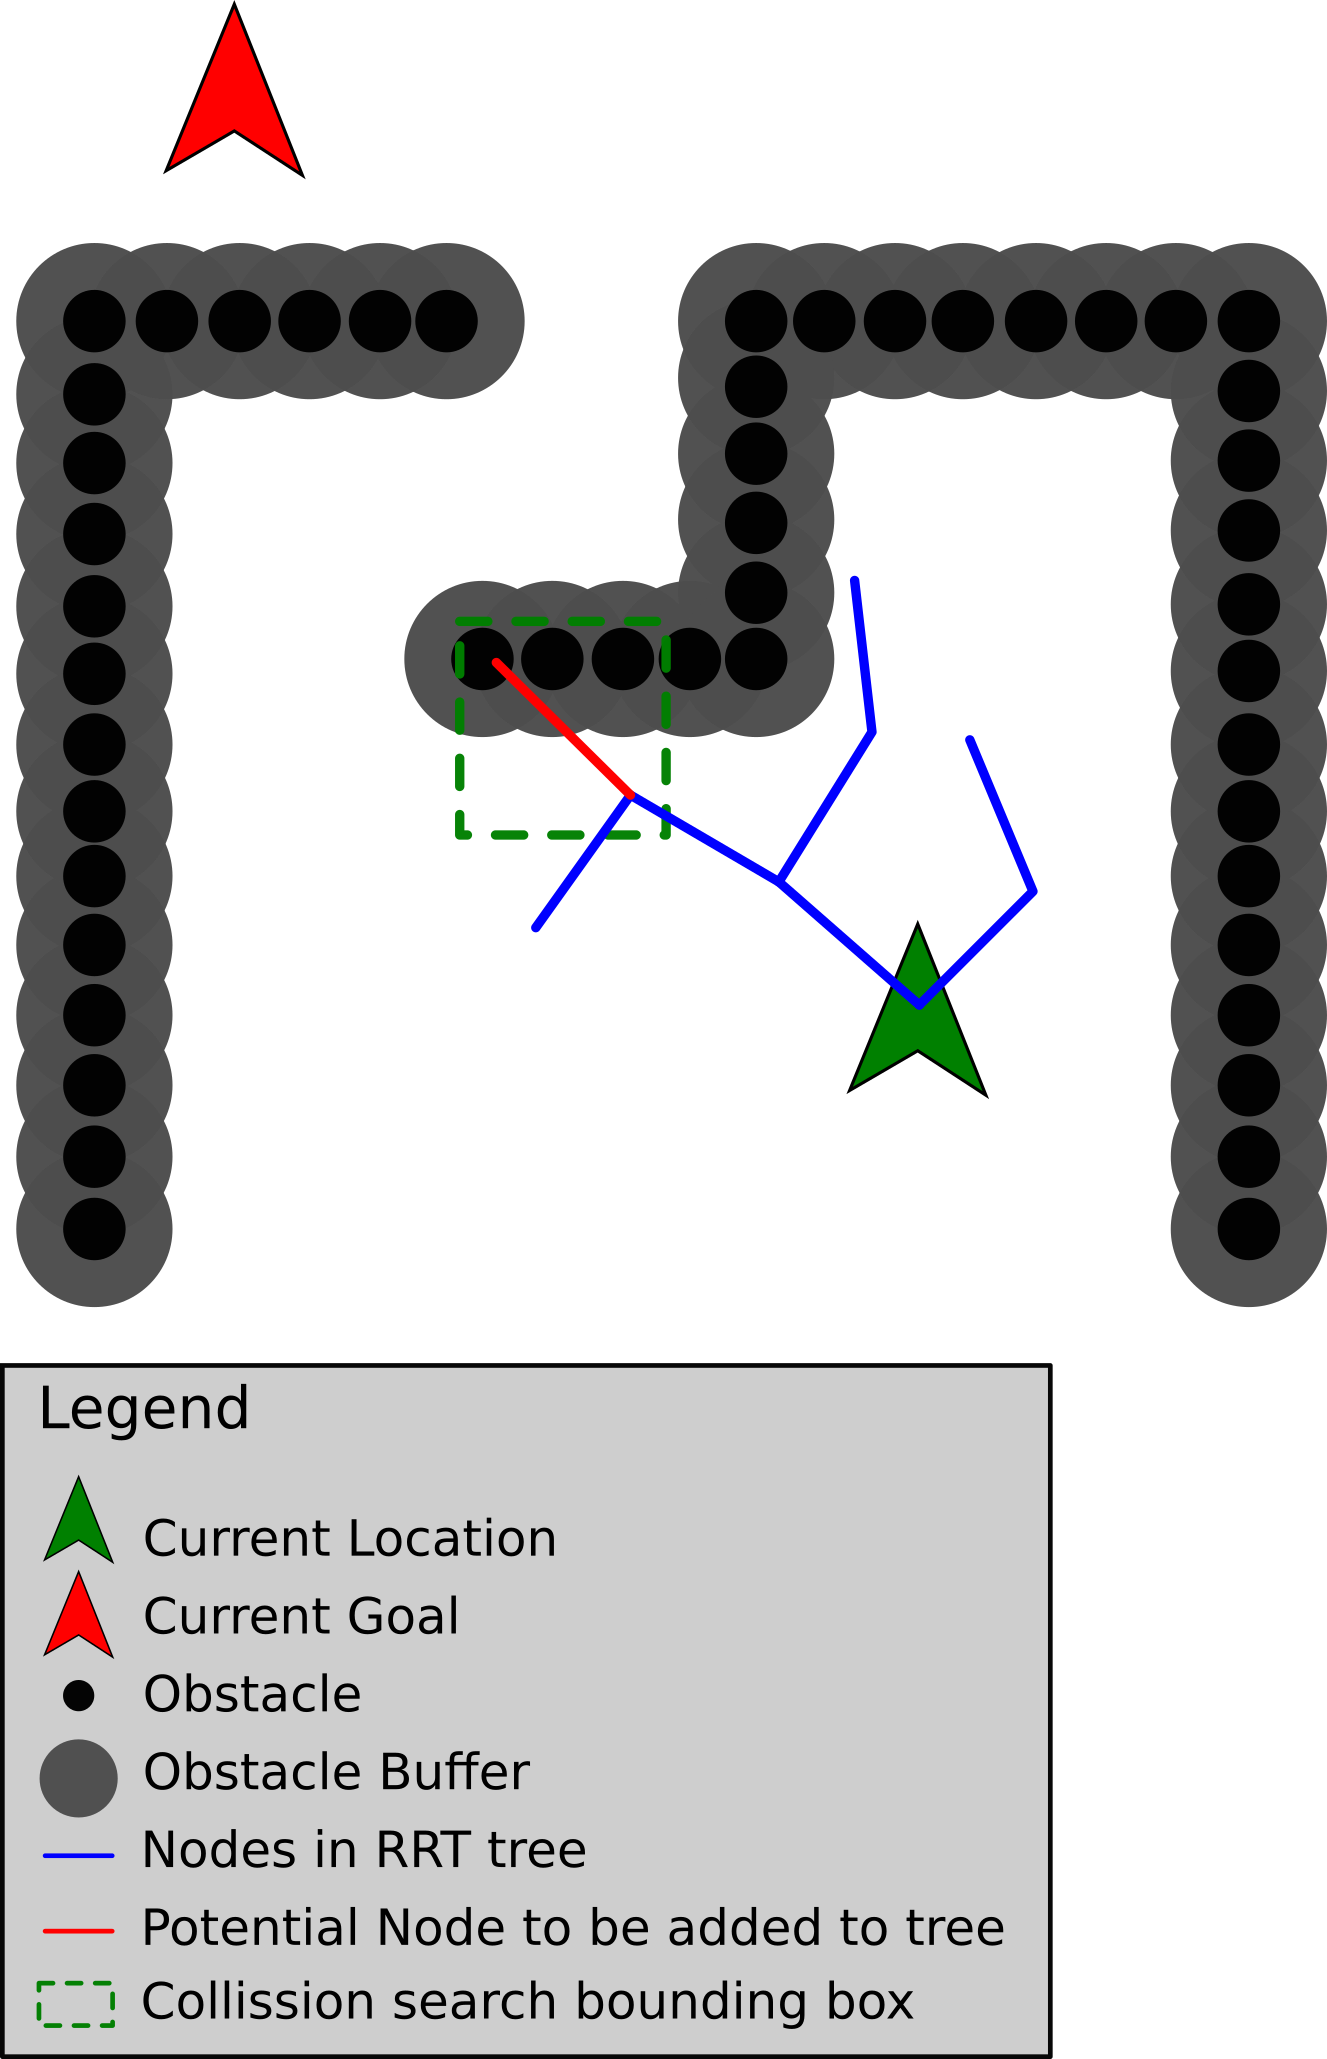
\includegraphics[width=0.8\linewidth]{rrt_sample}
\caption{Example of one step of collision check with the RRT planner.}
\label{fig:rrt_sample}
\end{figure}

As the RRT branches propagate, before each candidate node is added to the tree, an obstacle collision check is done only on the obstacles within range of the new node. The obstacles are determined to be in range according to algorithm \ref{dyn_path_plan}.

\begin{algorithm}
  \caption{Obstacle Range Filter}
  \label{dyn_path_plan}
\begin{algorithmic}
  \REQUIRE $\mathit{candidate\_branch}$, $\mathit{obstacle\_list}$, $r_{\mathit{buf}}$
  \FORALL{$\mathit{obstacles}$ in $\mathit{obstacle\_list}$}
    \IF{$x_{\mathit{obs}} + r_{\mathit{buf}} \leq \min{(x_1, x_2)}$}
      \STATE continue
    \ELSIF{$x_{\mathit{obs}} - r_{\mathit{buf}} \geq \max{(x_1, x_2)}$}
      \STATE continue
    \ELSIF{$y_{\mathit{obs}} + r_{\mathit{buf}} \leq \min{(y_1, y_2)}$}
      \STATE continue
    \ELSIF{$y_{\mathit{obs}} - r_{\mathit{buf}} \geq \max{(y_1, y_2)}$}
      \STATE continue
    \ELSE
      \STATE $\mathit{filtered\_obstacles} \gets \mathit{obstacle}$
    \ENDIF
  \ENDFOR
  \RETURN $\mathit{filtered\_obstacles}$
\end{algorithmic}
\end{algorithm}

 The points $(x_1,y_1)$ and $(x_2,y_2)$ are the endpoints of the candidate branch, $(x_{\mathit{obs}},y_{\mathit{obs}})$ is the location of the obstacle being checked, and $r_{\mathit{buf}}$ is the buffer radius for each obstacle. The green bounding box in Fig. \ref{fig:rrt_sample} shows which obstacles would be included in the $\mathit{filtered\_obstacles}$ after this check. The perpendicular distance between the candidate line (shown in red) and each remaining obstacle is found by

\begin{equation}
  d = \dfrac{|\Delta y \; x_{\mathit{obs}} -
      \Delta x \; y_{\mathit{obs}} + \Delta s|}
      {\sqrt{\Delta y^2 + \Delta x^2}},\\
\end{equation}
  % \nonumber \text{where}\\
where
\begin{align}
  \Delta x &= x_2 - x_1\\
  \Delta y &= y_2 - y_1\\
  \Delta s &= x_2 \; y_1 -x_1 \; y_2.
\end{align}

 If the distance $d$ is less than the buffer radius, a collision is detected and the candidate is rejected. By only checking for collisions with obstacles within the bounding box, nearly all obstacles are ignored for each step of propagation. This significantly improves performance of the RRT planner and allows it to plan in real-time and dynamically update the path whenever needed. The collision detection for path smoothing and path checking works the same way, with $(x_1,y_1)$ and $(x_2,y_2)$ being the endpoints of each path segment.

% \subsection{Path Planning Algorithm}
% The path planning breaks down to four separate functions. The RRT planner, collision checker, path smoother, and path checker. Each time the obstacles are updated, the path checker is run to see if the current path is still valid. If invalid, the RRT planner is run from the current location then the path is smoothed following the
%
%
% \begin{algorithm}
%   \caption{Dynamic Path Planner}
%   \label{dyn_path_plan}
% \begin{algorithmic}
%     \IF{some condition is true}
%         \STATE do some processing
%     \ELSIF{some other condition is true}
%         \STATE do some different processing
%     \ELSE
%         \STATE do the default actions
%     \ENDIF
% \end{algorithmic}
% \end{algorithm}
%
%
% \todo{include algorithm section to explain what the planner is doing? or just more explanation? or is this good enough?}

%%%%%%%%%%%%%%%%%%%%%%%%%%%%%%%%%%%%%%%%%%%%%%%%%%%%%%%%%%%%%%%%%%%%%%%%%%%%%%%%
\section{Map Merging}\label{nav_merge}

The map merging process we use is able to generate a combined map from multiple agents on a base-station computer in near real-time as the UAVs are mapping the environment. Fig. \ref{fig:map_merge} shows the network diagram of the process of merging the maps. To merge the maps in near real-time, each time a new keyframe is initialized, its data is stored in the RGB-D Cache database which is hosted on the base-station computer. A 3D color and depth (XYZRGB) pointcloud is generated using the color and depth information from the RGB-D cameras and the features are generated from either SIFT/SURF or ORB using OpenCV.

\begin{figure*}
\centering
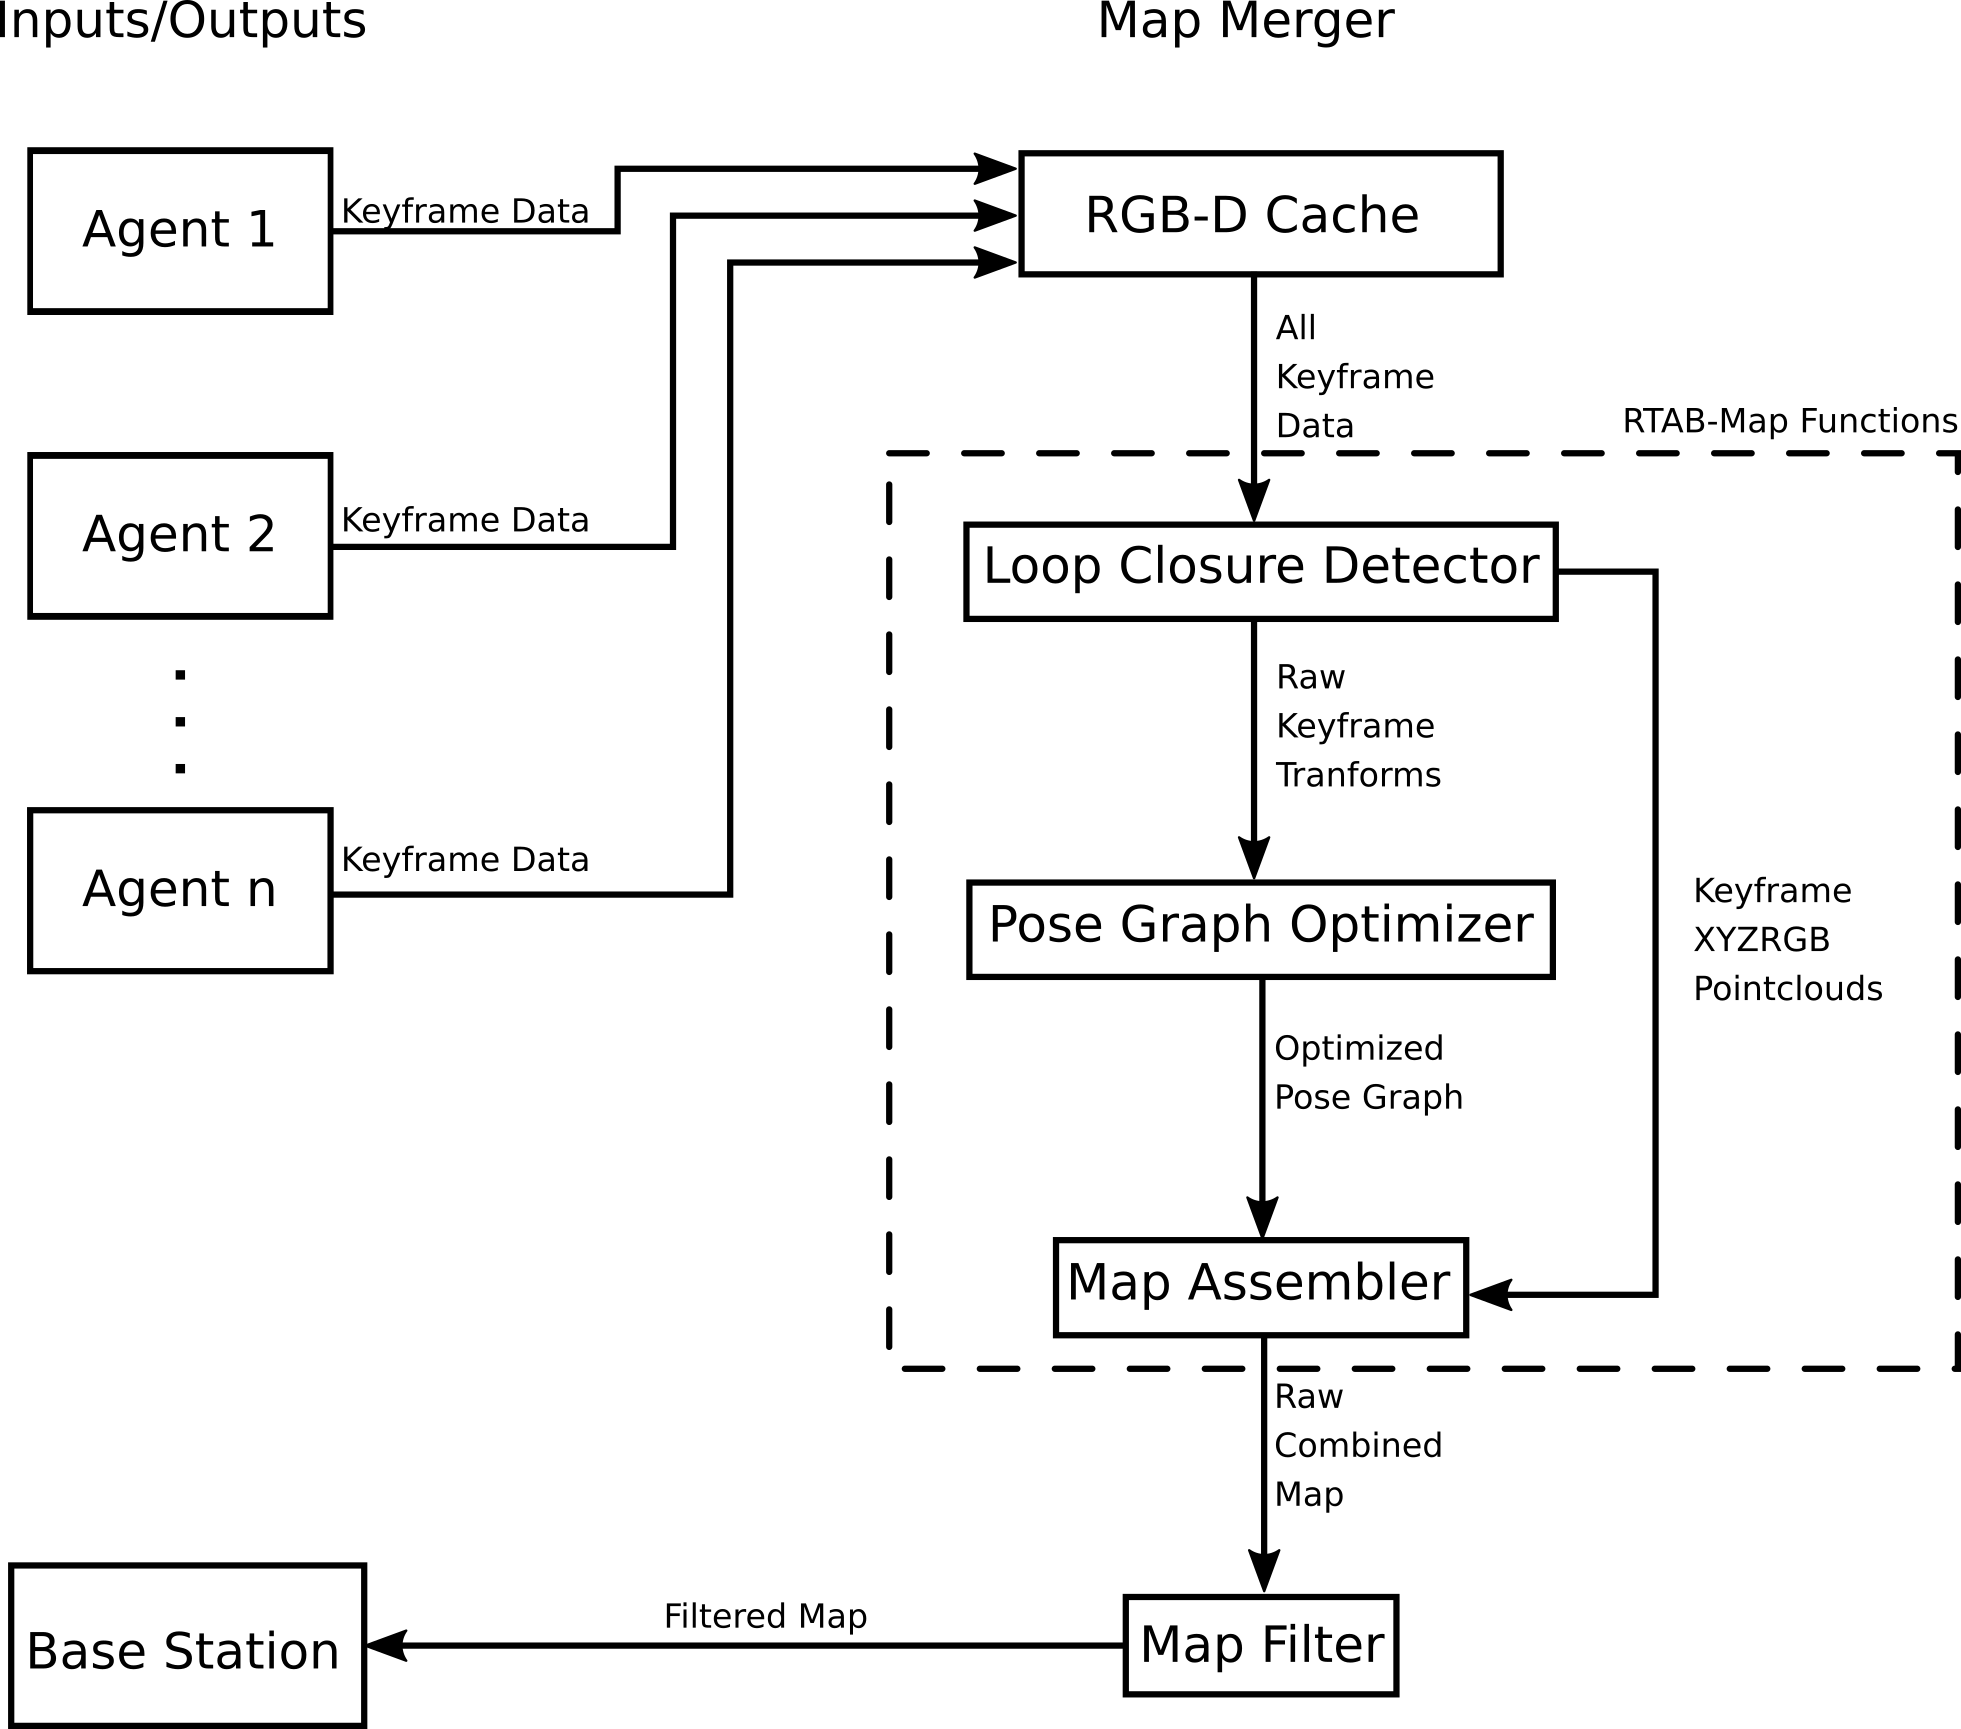
\includegraphics[width=0.8\linewidth]{map_merger_network}
\caption[The network diagram for the multi-agent map merging node.]{The network diagram for the multi-agent map merging node proposed in this section.}
\label{fig:map_merge}
\end{figure*}

Once the database has been initialized, the maps are periodically merged using functions from an instance of RTAB-Map running on the base-station computer. This merging process functions similarly to how individual maps are generated for each UAV \cite{Labbe2011a,Labbe2013,Labbe2019}. The first step is to search for loop closures in the feature descriptions from each keyframe using a bag-of-words approach. Rather than only look for loop closures from the keyframes of a single agent, this process looks for loop closures from all keyframes from all agents. Each time a new loop closure is found, a new edge is added to combined map graph with an estimated transformation between keyframes. After finding all loop closures with the current dataset, the graph is optimized using the pose graph optimizer built into RTAB-Map. The optimized pose graph is then sent to the map assembler along with the XYZRGB pointcloud from each keyframe where the pointclouds are combined according to the optimized graph edges. This generates a single map with all keyframes that can be connected into a single graph. This map is then processed to reduce noise and filter out the ceiling to make the map more understandable to the operator.

Since the base-station computer is merging the maps, the algorithm is able to run in real-time. The larger the map grows, the longer it takes to re-optimize the the combined map. This causes the updated map to lag behind real-time when the map is large.
%%%%%%%%%%%%%%%%%%%%%%%%%%%%%%%%%%%%%%%%%%%%%%%%%%%%%%%%%%%%%%%%%%%%%%%%%%%%%%%%
\section{Results and Discussion}\label{nav_results}

\subsection{Simulation}

We successfully navigated and mapped a simulation environment autonomously in ROS Gazebo \cite{OSRF} with multiple agents and combined the maps. The simulation environment was designed to be as close to the real world and hardware as possible. We used a software-in-the-loop (SIL) version of ROSflight \cite{Jackson2016a}, an open-source autopilot library built with ROS, to mimic the flight controller. We did not use any ground-truth information in the simulation; all measurements were from simulated sensors with noise characteristics similar to hardware. Fig. \ref{fig:sim_setup} shows the simulation setup used to map the environment.

\begin{figure}
\centering
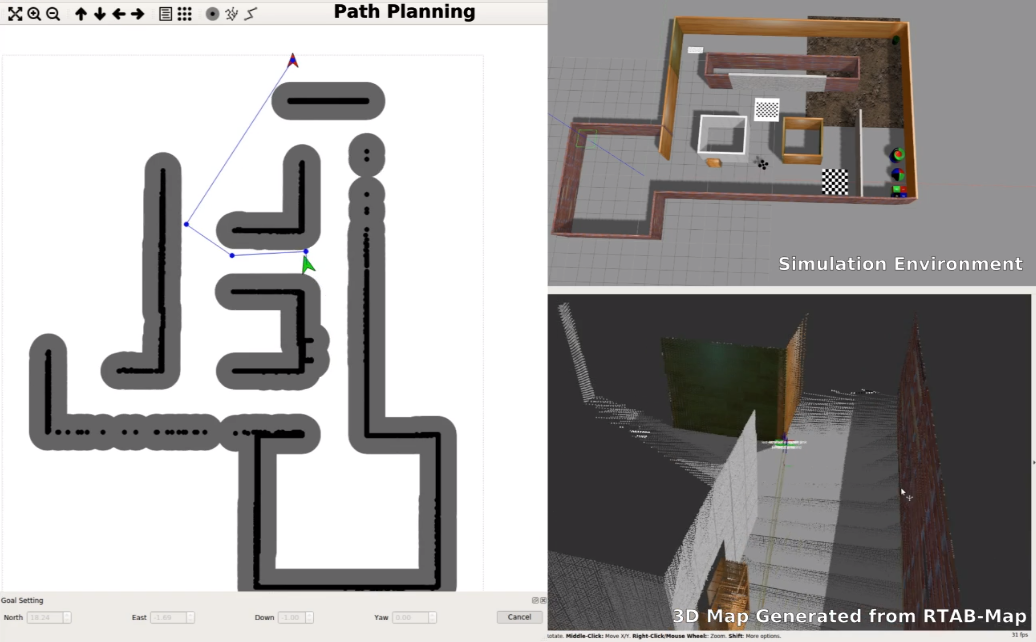
\includegraphics[width=1.0\linewidth]{sim_setup}
\caption[Setup used for map merging simulation results.]{Setup used for the simulation results. The reactive planner is shown on the left, the simulation world is shown on the top right, and the current map is shown on the bottom right.}
\label{fig:sim_setup}
\end{figure}

Fig. \ref{fig:sim_map} shows the results from mapping the simulated environment with two agents and combining the maps. Neither agent saw everything in the combined map, but the maps were successfully merged together into a single map with all features from each individual map.

\begin{figure*}
\centering
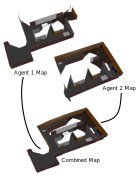
\includegraphics[width=0.7\linewidth]{sim_map}
\caption{Map generated from combined maps in the simulated environment.}
\label{fig:sim_map}
\end{figure*}

Flying in simulation helped validate the reactive planner and obstacle avoidance. It was also helpful to debug and sort out the communication architecture of the relative navigation framework and control schemes. The area where the simulation falls short is with the computer vision applications such as visual odometry and loop-closure detection. Gazebo is excellent at simulating realistic physics and dynamics, but the environments are significantly less detailed than the real world. This makes designing a simulation world more difficult. If there is too little detail added to the world, the visual odometry algorithms often fail or perform poorly. If too much repetitive detail is used, RTAB-Map finds too many false loop closures and the mapping fails. The simulated world developed and used to obtain results as shown in Figs. \ref{fig:sim_setup} and \ref{fig:sim_map} is able to minimize these issues, but still failed to produce results on par with a real world test. There were only a few locations in the simulated world with enough unique detail that loop closures were reliably detected. In contrast, a real world environment has enough detail that loop closures can be detected nearly everywhere except for large blank walls and glass. After proving the setup in a high-fidelity simulation, we moved to hardware to more thoroughly test the computer vision aspects of the approach

\subsection{Hardware}

The extension of RTAB-Map to enable real-time map merging of multiple UAVs flying simultaneously is robust enough to handle several vehicles at the same time. We began testing with only two vehicles and were able to expand it up to four vehicles. We were able to successfully combine maps generated from multiple UAVs in near real time with manual flight. Fig. \ref{fig:wilk3_map} shows an example of a map built from a an indoor environment with with both hallways and large rooms. The generated map is sufficiently dense to show detail for a human user to interpret and get actionable information. This map was built from manually flying a single UAV four times and recording the data, then playing back all data simultaneously and merging the map in real time as shown in Fig. \ref{fig:map_seq}. By the end of the map merging process with this data, the combined map generation was lagging behind real-time by about one minute. There is theoretically no limit to the number of vehicles that could be added and flown simultaneously, but as more vehicles are added, the merging process lags further behind real time and loop closure detection gets more complex.

\begin{figure*}
\centering
\includegraphics[width=1.0\linewidth]{wilk3_manual.png}
\caption[Map generated from four combined maps in hardware manual flight.]{Example of hardware results of merging maps from four agents into a single map in an indoor environment. Above the individual agent maps are examples of the detail in the pointclouds when zoomed in.}
\label{fig:wilk3_map}
\end{figure*}

\begin{figure*}
\centering
\includegraphics[width=1.0\linewidth]{map_merge_sequence.png}
\caption[An example of the map merging process over time.]{Example of the merged map being generated in near real-time. The combined map is updated every 30-40 seconds as agents are flying.}
\label{fig:map_seq}
\end{figure*}

%%%%%%%%%%%%%%%%%%%%%%%%%%%%%%%%%%%%%%%%%%%%%%%%%%%%%%%%%%%%%%%%%%%%%%%%%%%%%%%%
\section{Conclusions}\label{nav_conclusions}

Using UAVs to generate dense 3D maps of GPS-denied environments requires a careful choice of planning, estimation, and mapping techniques to be successful. Using the combination of a reactive path planner and a CEPA obstacle avoidance velocity filter allows for navigation and exploration through complex GPS-denied environments. Estimating relative and global states separately allows for the necessary decoupling of position and attitude controllers to fly autonomously without the use of GPS. Using multiple UAVs to collaboratively map an area improves mapping efficiency and, when handled correctly, still allows the map building to occur in near real-time. Future work includes streamlining the map merging process to allow for full real-time map generation, and connecting the UAVs to a high-level coverage path planner to allow for fully autonomous flight without human guidance.

%%%%%%%%%%%%%%%%%%%%%%%%%%%%%%%%%%%%%%%%%%%%%%%%%%%%%%%%%%%%%%%%%%%%%%%%%%%%%%%%
\section{Acknowledgements}
Thanks to Mathieu Labbe for being responsive to answering questions on the RTAB-Map forum and helping with developing the map merging node. This research was funded by The National Institute of Standards and Technology (NIST) under award number 70NANB17H211.

%%%%%%%%%%%%%%%%%%%%%%%%%%%%%%%%%%%%%%%%%%%%%%%%%%%%%%%%%%%%%%%%%%%%%%%%%%%%%%%%
\bibliographystyle{IEEEtran} % We choose the "plain" reference style
\bibliography{clean_refs}

\end{document}
